\section{Mustererkennung (Ravell Heerdegen)} \label{Mustererkennung}
Pattern recognition zeichnet sich durch die Möglichkeit aus, Klassifizierungen durchzuführen. Die Klassifizierungen sind entweder überwacht oder frei von Überwachung. Das bedeutet, dass die Klassifizierungen automatisch oder mit menschlicher Hilfe ablaufen können \cite{svmgmm}. Im Bereich pattern recognition haben sich besonders neuronale Netze als enormer Fortschritt herausgestellt. Mit neuronalen Netzen werden u.a.~Muster in Daten erkannt und zugeordnet. Auch können Gefühle aus Gesichtern heraus analysiert und zwischen mehreren Personen und ihrer Position in einem Bild unterschieden werden. Des Weiteren können Merkmale erkannt und spezifischen Klassen zugeordnet werden, oder auch Bewertungen von Performanz durchgeführt werden~\cite{patternrec}.
In diesem Kapitel wird zunächst auf CNNs eingegangen, da CNNs in den folgenden Beispielen priorisiert zum Einsatz kommen. Danach wird die Disziplin speech recognition anhand von drei Beispielen erläutert. Anschließend wird die Disziplin emotion recognition mithilfe von zwei Beispielen näher beleuchtet.
\\
\subsection{Convolutional neural networks}
CNNs sind sogenannte feed-forward neural networks. Das bedeutet, dass Signale wie z.B.~Geräusche durch die verschiedenen Layer (Schichten) des neuronalen Netzes (NN) gegeben werden. CNNs können in voller Ausführung aus input layers, convolutional layers, pooling layers, sowie fully-connected layers und output layers bestehen~\cite{facialemotionrecusingcnn}. Jeder Layer besteht aus einer Vielzahl von zweidimensionalen Flächen. Eine Fläche besitzt mehrere unabhängige Neuronen.
\\
\\
\\
\begin{figure}[h]
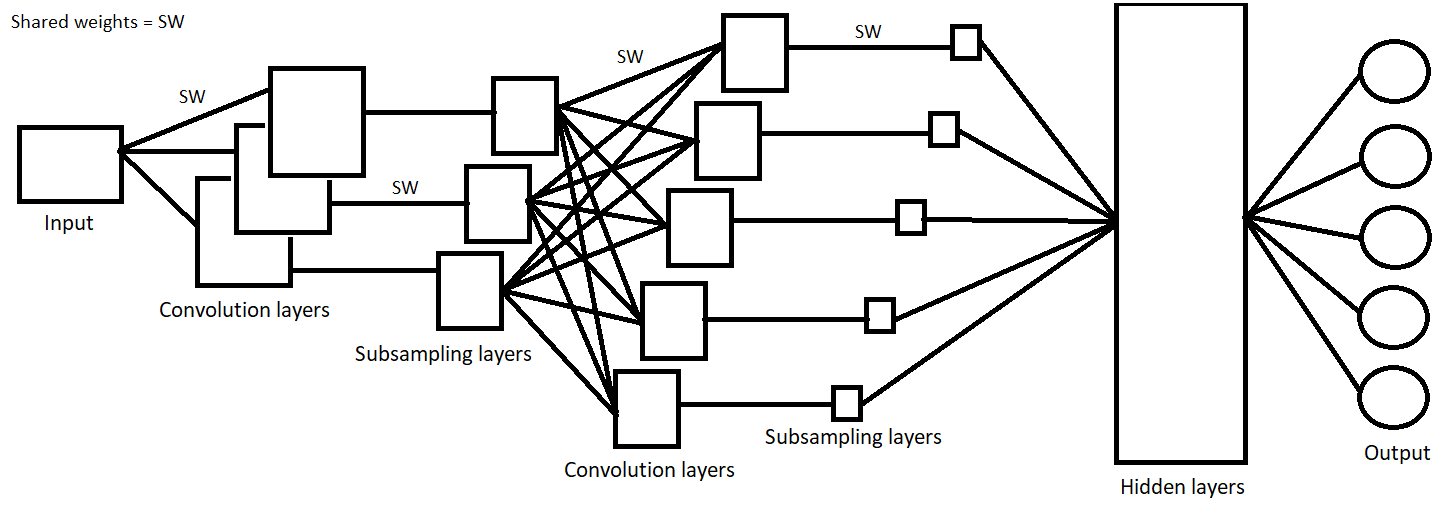
\includegraphics[width=\linewidth, height=6cm]{Bilder/CNN/CNNArchitektur.png}
\caption{CNN-Architektur vgl.~\cite{noisycnn}}
\end{figure}
\\
Spracheingaben werden in eine bestimmte Menge an Frequenzen unterteilt. Jede einzelne Frequenz wird mit sogenannten Gewichten verglichen, welche mit einer lokalen Variable im Layer multipliziert werden. Die Gewichte werden auf den gesamten Eingaberaum verteilt. Die Verteilung aktiviert die convolutional layers und teilt diese in verschiedene Bereiche auf. Jeder convolutional layer besitzt diverse Filter. Durch die Filter entstehen sogenannte hidden units. Hidden units sind beschreibbare Plätze auf einem Layer. Im Anschluss werden die hidden units in einen max-pooling layer gegeben. Im max-pooling layer werden Varianzen, also Abweichungen der einzelnen hidden units entfernt. Die Varianzen können u.a.~aus Dialekten, undeutlicher Sprache oder Störungen in der Übertragung kommen. Die nun bereinigten hidden units werden in den convolutional layers als Trainingsparameter eingespeichert. Somit erkennt jeder convolutional layer verschiedene Merkmale, aufgrund der ihm zur Verfügung stehenden Merkmalsammlung~\cite{usingcnn}.